% Options for packages loaded elsewhere
\PassOptionsToPackage{unicode}{hyperref}
\PassOptionsToPackage{hyphens}{url}
%
\documentclass[
]{article}
\usepackage{amsmath,amssymb}
\usepackage{iftex}
\ifPDFTeX
  \usepackage[T1]{fontenc}
  \usepackage[utf8]{inputenc}
  \usepackage{textcomp} % provide euro and other symbols
\else % if luatex or xetex
  \usepackage{unicode-math} % this also loads fontspec
  \defaultfontfeatures{Scale=MatchLowercase}
  \defaultfontfeatures[\rmfamily]{Ligatures=TeX,Scale=1}
\fi
\usepackage{lmodern}
\ifPDFTeX\else
  % xetex/luatex font selection
\fi
% Use upquote if available, for straight quotes in verbatim environments
\IfFileExists{upquote.sty}{\usepackage{upquote}}{}
\IfFileExists{microtype.sty}{% use microtype if available
  \usepackage[]{microtype}
  \UseMicrotypeSet[protrusion]{basicmath} % disable protrusion for tt fonts
}{}
\makeatletter
\@ifundefined{KOMAClassName}{% if non-KOMA class
  \IfFileExists{parskip.sty}{%
    \usepackage{parskip}
  }{% else
    \setlength{\parindent}{0pt}
    \setlength{\parskip}{6pt plus 2pt minus 1pt}}
}{% if KOMA class
  \KOMAoptions{parskip=half}}
\makeatother
\usepackage{xcolor}
\usepackage{graphicx}
\makeatletter
\def\maxwidth{\ifdim\Gin@nat@width>\linewidth\linewidth\else\Gin@nat@width\fi}
\def\maxheight{\ifdim\Gin@nat@height>\textheight\textheight\else\Gin@nat@height\fi}
\makeatother
% Scale images if necessary, so that they will not overflow the page
% margins by default, and it is still possible to overwrite the defaults
% using explicit options in \includegraphics[width, height, ...]{}
\setkeys{Gin}{width=\maxwidth,height=\maxheight,keepaspectratio}
% Set default figure placement to htbp
\makeatletter
\def\fps@figure{htbp}
\makeatother
\setlength{\emergencystretch}{3em} % prevent overfull lines
\providecommand{\tightlist}{%
  \setlength{\itemsep}{0pt}\setlength{\parskip}{0pt}}
\setcounter{secnumdepth}{-\maxdimen} % remove section numbering
\ifLuaTeX
  \usepackage{selnolig}  % disable illegal ligatures
\fi
\IfFileExists{bookmark.sty}{\usepackage{bookmark}}{\usepackage{hyperref}}
\IfFileExists{xurl.sty}{\usepackage{xurl}}{} % add URL line breaks if available
\urlstyle{same}
\hypersetup{
  pdftitle={Macro Spring 1 Essay 2},
  hidelinks,
  pdfcreator={LaTeX via pandoc}}

\title{Macro Spring 1 Essay 2}
\author{}
\date{}

\begin{document}
\maketitle

\hypertarget{using-economic-theory-discuss-the-determinants-of-gdp-per-capita-in-the-long-run-and-the-growth-rate-of-gdp-per-capita-in-the-long-run.-examine-how-these-two-phenomena-respond-to-a-permanent-decrease-in-the-growth-rate-of-the-population.}{%
\section{Using Economic Theory Discuss the Determinants of GDP per
Capita in the Long-run, and the Growth Rate of GDP per Capita in the
Long-run. Examine how These Two Phenomena Respond to a Permanent
Decrease in the Growth Rate of the
Population.}\label{using-economic-theory-discuss-the-determinants-of-gdp-per-capita-in-the-long-run-and-the-growth-rate-of-gdp-per-capita-in-the-long-run.-examine-how-these-two-phenomena-respond-to-a-permanent-decrease-in-the-growth-rate-of-the-population.}}

\begin{center}\rule{0.5\linewidth}{0.5pt}\end{center}

GDP per capita is a measure of total economic output for each person in
an economy. Unlike the short run, the determinants of long run GDP per
capita are less influenced by cyclical or temporary fluctuations within
the economy, such as fluctuations in prices of changes in fiscal or
monetary policy, instead, more structural indicators are needed to
determine GDP per capita in the long run. In modern economic theory,
there are three main contributing factors to long run GDP per capita
growth.

Firstly, capital accumulation, defined as the total physical stock of
capital, this is an aggregate of all the machinery, factories, office
spaces, et cetera, within an economy. A higher level of capital stock is
associated with long run GDP per capita growth as it increases the
productivity of each worker, thus allowing an economy to expand its
production possibility frontier, and causing greater long run GDP per
capita. Secondly, size of labour force, defined as the total number of
people willing and able to work within an economy (Blanchard, 2017), a
greater labour force allows for more products to be made. However, it
must be considered that the labour force itself is included within the
per capita measurement of GDP, therefore, an expansion of the labour
force that coincides with overall population growth may not necessarily
result in an increase of GDP per capita if there is diminishing returns
to scale. Due to the marginal output per worker being less than one,
adding an additional worker would result in less additional output than
the previous worker, thus resulting in a reduction in overall output per
capita. Consequently, it may be better to use labour force
participation, as an increase in the proportion of the population
working increases output per worker. Thirdly, technological progress.
Defined as the discovery of new and improved methods of producing goods,
changes in technology lead to an increase in productivity of all factors
of production including labour and capital (CFI, 2022). By increasing in
the quality of capital, this allows for greater productivity by reducing
the value of capital needed for each worker to produce the same amount
as previously. Furthermore, technological progress allows for new
products which are of greater value then before, hence producing these
output increases overall GDP per capita in the long run.

In order to examine how these phenomena react to a permanent decrease in
population growth we must establish a model to derive how these
determinants react to each other. The Solow-Swan growth model is used to
predict the impact of factor inputs on output (GDP) per capita. The
model establishes a theoretical one-good economy and a production
function with constant returns to scale, whilst also allowing capital
and labour to be substituted for each other in the ratio of each others
marginal product. Hence, Solow\textquotesingle s production function is
a many to one mapping of capital and labour to output:

{\[\begin{matrix}
{Y = F(K,N)} \\
\end{matrix}\]}

Since there is constant returns to scale, any proportional change in
both capital and labour would result in the same proportional change in
output. For example, doubling of both capital and number of workers
would result in a doubling of output. This can be described as,

{\[\begin{matrix}
{xY = F(xK,xN)} \\
\end{matrix}\]}

To account for technological progress, the model appends a coefficient
to the number of workers, {\(A\)}, which refers to the state of
technology in the economy:

{\[\begin{matrix}
{Y = F(K,AN)} \\
\end{matrix}\]}

The implication that follows is that for any doubling of the state of
technology has explicitly the same impact of doubling the number of
workers. In practice, this holds as innovation that doubles the marginal
output per worker would result in half as many workers needed to make
the same number of goods. {\(AN\)} henceforth will be referred to as
effective workers, as it implies the amount of workers needed to produce
the same output without current state of technology: 1 worker with
technology that doubles their output is \emph{effectively} the same as 2
workers without said technology.

Since it is established that there is constant returns to scale, we can
set {\(x\)} from equation {\((2)\)} equal the reciprocal of effective
workers {\(\frac{1}{AN}\)} thus creating out per effective capita
production function:

\[\begin{matrix}
\begin{matrix}
\frac{Y}{AN} & {= F\left( \frac{K}{AN},\frac{AN}{AN} \right)} \\
 & {= F\left( \frac{K}{AN},1 \right)} \\
 & {= f\left( \frac{K}{AN} \right)} \\
\end{matrix} \\
\end{matrix}\]

\hypertarget{here-the-aggregate-production-function-is-essentially-divided-by-the-number-of-effective-workers-an-itself-becomes-a-constant-since-fracanan-is-1-and-thus-not-a-determinant-in-the-output-per-capita-aggregate-production-function.-for-simplicity-this-relationship-can-be-expressed-as-function-fleft-frackan-right.-to-establish-an-equi-using-economic-theory-discuss-the-determinants-of-gdp-per-capita-in-the-long-run-and-the-growth-rate-of-gdp-per-capita-in-the-long-run.-examine-how-these-two-phenomena-respond-to-a-permanent-decrease-in-the-growth-rate-of-the-population.}{%
\subsection{\texorpdfstring{Here, the aggregate production function is
essentially divided by the number of effective workers, {\(AN\)} itself
becomes a constant since {\(\frac{AN}{AN}\)} is 1, and thus not a
determinant in the output per capita aggregate production function. For
simplicity, this relationship can be expressed as function
{\(f\left( \frac{K}{AN} \right)\)}. To establish an equi\# Using
Economic Theory Discuss the Determinants of GDP per Capita in the
Long-run, and the Growth Rate of GDP per Capita in the Long-run. Examine
how These Two Phenomena Respond to a Permanent Decrease in the Growth
Rate of the
Population.}{Here, the aggregate production function is essentially divided by the number of effective workers, AN itself becomes a constant since \textbackslash frac\{AN\}\{AN\} is 1, and thus not a determinant in the output per capita aggregate production function. For simplicity, this relationship can be expressed as function f\textbackslash left( \textbackslash frac\{K\}\{AN\} \textbackslash right). To establish an equi\# Using Economic Theory Discuss the Determinants of GDP per Capita in the Long-run, and the Growth Rate of GDP per Capita in the Long-run. Examine how These Two Phenomena Respond to a Permanent Decrease in the Growth Rate of the Population.}}\label{here-the-aggregate-production-function-is-essentially-divided-by-the-number-of-effective-workers-an-itself-becomes-a-constant-since-fracanan-is-1-and-thus-not-a-determinant-in-the-output-per-capita-aggregate-production-function.-for-simplicity-this-relationship-can-be-expressed-as-function-fleft-frackan-right.-to-establish-an-equi-using-economic-theory-discuss-the-determinants-of-gdp-per-capita-in-the-long-run-and-the-growth-rate-of-gdp-per-capita-in-the-long-run.-examine-how-these-two-phenomena-respond-to-a-permanent-decrease-in-the-growth-rate-of-the-population.}}

GDP per capita is a measure of total economic output for each person in
an economy. Unlike the short run, the determinants of long run GDP per
capita are less influenced by cyclical or temporary fluctuations within
the economy, such as fluctuations in prices of changes in fiscal or
monetary policy, instead, more structural indicators are needed to
determine GDP per capita in the long run. In modern economic theory,
there are three main contributing factors to long run GDP per capita
growth.

Firstly, capital accumulation, defined as the total physical stock of
capital, this is an aggregate of all the machinery, factories, office
spaces, et cetera, within an economy. A higher level of capital stock is
associated with long run GDP per capita growth as it increases the
productivity of each worker, thus allowing an economy to expand its
production possibility frontier, and causing greater long run GDP per
capita. Secondly, size of labour force, defined as the total number of
people willing and able to work within an economy (Blanchard, 2017), a
greater labour force allows for more products to be made. However, it
must be considered that the labour force itself is included within the
per capita measurement of GDP, therefore, an expansion of the labour
force that coincides with overall population growth may not necessarily
result in an increase of GDP per capita if there is diminishing returns
to scale. Due to the marginal output per worker being less than one,
adding an additional worker would result in less additional output than
the previous worker, thus resulting in a reduction in overall output per
capita. Consequently, it may be better to use labour force
participation, as an increase in the proportion of the population
working increases output per worker. Thirdly, technological progress.
Defined as the discovery of new and improved methods of producing goods,
changes in technology lead to an increase in productivity of all factors
of production including labour and capital (CFI, 2022). By increasing in
the quality of capital, this allows for greater productivity by reducing
the value of capital needed for each worker to produce the same amount
as previously. Furthermore, technological progress allows for new
products which are of greater value then before, hence producing these
output increases overall GDP per capita in the long run.

In order to examine how these phenomena react to a permanent decrease in
population growth we must establish a model to derive how these
determinants react to each other. The Solow-Swan growth model is used to
predict the impact of factor inputs on output (GDP) per capita. The
model establishes a theoretical one-good economy and a production
function with constant returns to scale, whilst also allowing capital
and labour to be substituted for each other in the ratio of each others
marginal product. Hence, Solow\textquotesingle s production function is
a many to one mapping of capital and labour to output:

{\[\begin{matrix}
{Y = F(K,N)} \\
\end{matrix}\]}

Since there is constant returns to scale, any proportional change in
both capital and labour would result in the same proportional change in
output. For example, doubling of both capital and number of workers
would result in a doubling of output. This can be described as,

{\[\begin{matrix}
{xY = F(xK,xN)} \\
\end{matrix}\]}

To account for technological progress, the model appends a coefficient
to the number of workers, {\(A\)}, which refers to the state of
technology in the economy:

{\[\begin{matrix}
{Y = F(K,AN)} \\
\end{matrix}\]}

The implication that follows is that for any doubling of the state of
technology has explicitly the same impact of doubling the number of
workers. In practice, this holds as innovation that doubles the marginal
output per worker would result in half as many workers needed to make
the same number of goods. {\(AN\)} henceforth will be referred to as
effective workers, as it implies the amount of workers needed to produce
the same output without current state of technology: 1 worker with
technology that doubles their output is \emph{effectively} the same as 2
workers without said technology.

Since it is established that there is constant returns to scale, we can
set {\(x\)} from equation {\((2)\)} equal the reciprocal of effective
workers {\(\frac{1}{AN}\)} thus creating out per effective capita
production function:

\[\begin{matrix}
\begin{matrix}
\frac{Y}{AN} & {= F\left( \frac{K}{AN},\frac{AN}{AN} \right)} \\
 & {= F\left( \frac{K}{AN},1 \right)} \\
 & {= f\left( \frac{K}{AN} \right)} \\
\end{matrix} \\
\end{matrix}\]

Here, the aggregate production function is essentially divided by the
number of effective workers, {\(AN\)} itself becomes a constant since
{\(\frac{AN}{AN}\)} is 1, and thus not a determinant in the output per
capita aggregate production function. For simplicity, this relationship
can be expressed as function {\(f\left( \frac{K}{AN} \right)\)}. To
establish an equilibrium output per worker (the steady-state output) we
must determine the factors that change capital per worker over a period
of time.

Allowing for technological progress, the number of effective workers
increases over time. Consequently, to retain the existing ratio of
capital to effective workers, {\(\frac{K}{AN}\)}, an increase in the
capital stock {\(K\)} proportional to an increase in the number of
effective workers {\(AN\)} is needed. Furthermore, the capital stock
depreciates over time as the value of machinery decreases and repairs
need to be made. Therefore, additional investment, on top of that needed
to retain the capital to effective worker ratio, is needed to prevent
the value of capital stock deteriorating over time due to depreciation.
Also, the growth rate of workers impacts the ratio of capital to
effective worker; if over a period of time the number of workers
decrease, then less investment is required to retain the current ratio
of capital to effective worker. Combining these determinants, the value
of future capital stock {\(K_{t + 1}\)} can be derived:
{\[\frac{K_{t + 1}}{AN} = (1 - \delta + g_{N} + g_{A})\frac{K_{t}}{AN} + \frac{I_{t}}{AN}\]}To
derive changes in capital stock over time, {\(K_{t + 1} - K_{t}\)}, we
can subtract {\(K_{t}\)} from both sides of the relation:
{\[\frac{K_{t + 1}}{AN} - \frac{K_{t}}{AN} = (g_{N} + g_{A} - \delta)\frac{K_{t}}{AN} + \frac{I_{t}}{AN}\]}To
bridge the gap between changes in capital stock and output in the long
run, the investment-savings relation can be used, whereby in an economy
with no public sector, current investment {\(I_{t}\)} is equal to
savings: the savings rate {\(S\)} multiplied by output {\(Y\)}.
{\[I_{t} = sY_{t}\]}Inserting this into the capital stock relation,
{\[\frac{K_{t + 1}}{AN} - \frac{K_{t}}{AN} = (g_{N} + g_{A} - \delta)\frac{K_{t}}{AN} + \frac{sY_{t}}{AN}\]}Or
in terms of the per capita aggregate production function:
{\[\frac{K_{t + 1}}{AN} - \frac{K_{t}}{AN} = (g_{N} + g_{A} - \delta)\frac{K_{t}}{AN} + sf\left( \frac{K_{t}}{AN} \right)\]}

In response to what would happen if there were a permanent decrease in
the population growth rate, the coefficient {\(g_{N}\)} would decrease.
Consequently, this has the effect of flattening the capital accumulation
curve from {\(gn \rightarrow gn^{\prime}\)}. As a result, the capital
per effective worker increases from {\(K \rightarrow K^{\prime}\)} and
the output per worker increases from {\(Y \rightarrow Y^{\prime}\)} .
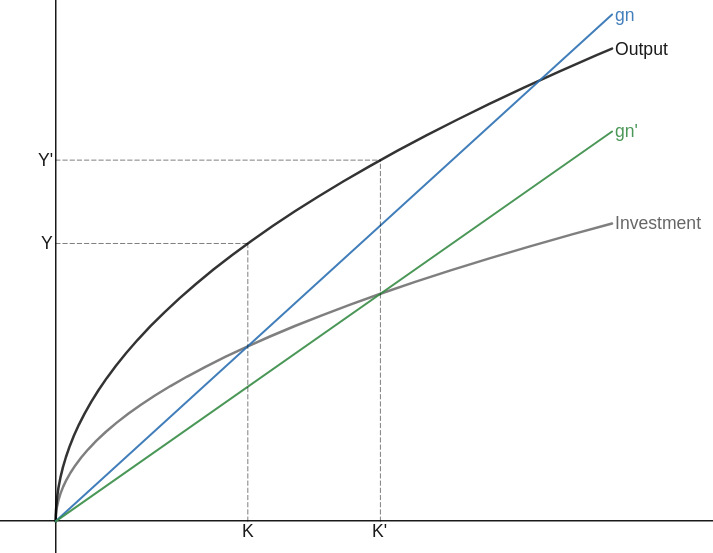
\includegraphics{/home/fontle/obsidian/Attachments/Pasted image 20230315151057.png}
\emph{(Beight-Welland, 2023)}

To conclude, we can see that a permanent decrease in population growth
would result in a increase in output per effective worker, and thus
overall GDP per capita. Furthermore, capital per worker increases since
if capital is accumulated at the same rate after the permanent
population decrease, more capital is available between fewer workers.

\hypertarget{bibliography}{%
\subsubsection{Bibliography}\label{bibliography}}

\begin{enumerate}
\tightlist
\item
  CFI. 2022, December 11, \emph{Technological Progress - Definition,
  Phases, How To Measure.} Corporatefinanceinstitute. {[}online{]}
  Available at:
  \url{https://corporatefinanceinstitute.com/resources/economics/technological-progress/}
  {[}Accessed 15 March. 2023{]}.
\item
  Blanchard, O \& Amighini, A \& Giavazzi, F. 2013,
  \emph{Macroeconomics: A European Perspective, Pearson Education UK,
  Harlow}. Available from: ProQuest Ebook Central. {[}15 March 2023{]}.
\item
  Beight-Welland, I. March 2023, \emph{Modelling Population Growth
  Change with the Solow Model}. Desmos. {[}online{]} Available at:
  \url{https://www.desmos.com/calculator/k48twmbzw2}
\end{enumerate}

librium output per worker (the steady-state output) we must determine
the factors that change capital per worker over a period of time.

Allowing for technological progress, the number of effective workers
increases over time. Consequently, to retain the existing ratio of
capital to effective workers, {\(\frac{K}{AN}\)}, an increase in the
capital stock {\(K\)} proportional to an increase in the number of
effective workers {\(AN\)} is needed. Furthermore, the capital stock
depreciates over time as the value of machinery decreases and repairs
need to be made. Therefore, additional investment, on top of that needed
to retain the capital to effective worker ratio, is needed to prevent
the value of capital stock deteriorating over time due to depreciation.
Also, the growth rate of workers impacts the ratio of capital to
effective worker; if over a period of time the number of workers
decrease, then less investment is required to retain the current ratio
of capital to effective worker. Combining these determinants, the value
of future capital stock {\(K_{t + 1}\)} can be derived:
{\[\frac{K_{t + 1}}{AN} = (1 - \delta + g_{N} + g_{A})\frac{K_{t}}{AN} + \frac{I_{t}}{AN}\]}To
derive changes in capital stock over time, {\(K_{t + 1} - K_{t}\)}, we
can subtract {\(K_{t}\)} from both sides of the relation:
{\[\frac{K_{t + 1}}{AN} - \frac{K_{t}}{AN} = (g_{N} + g_{A} - \delta)\frac{K_{t}}{AN} + \frac{I_{t}}{AN}\]}To
bridge the gap between changes in capital stock and output in the long
run, the investment-savings relation can be used, whereby in an economy
with no public sector, current investment {\(I_{t}\)} is equal to
savings: the savings rate {\(S\)} multiplied by output {\(Y\)}.
{\[I_{t} = sY_{t}\]}Inserting this into the capital stock relation,
{\[\frac{K_{t + 1}}{AN} - \frac{K_{t}}{AN} = (g_{N} + g_{A} - \delta)\frac{K_{t}}{AN} + \frac{sY_{t}}{AN}\]}Or
in terms of the per capita aggregate production function:
{\[\frac{K_{t + 1}}{AN} - \frac{K_{t}}{AN} = (g_{N} + g_{A} - \delta)\frac{K_{t}}{AN} + sf\left( \frac{K_{t}}{AN} \right)\]}

In response to what would happen if there were a permanent decrease in
the population growth rate, the coefficient {\(g_{N}\)} would decrease.
Consequently, this has the effect of flattening the capital accumulation
curve from {\(gn \rightarrow gn^{\prime}\)}. As a result, the capital
per effective worker increases from {\(K \rightarrow K^{\prime}\)} and
the output per worker increases from {\(Y \rightarrow Y^{\prime}\)} .
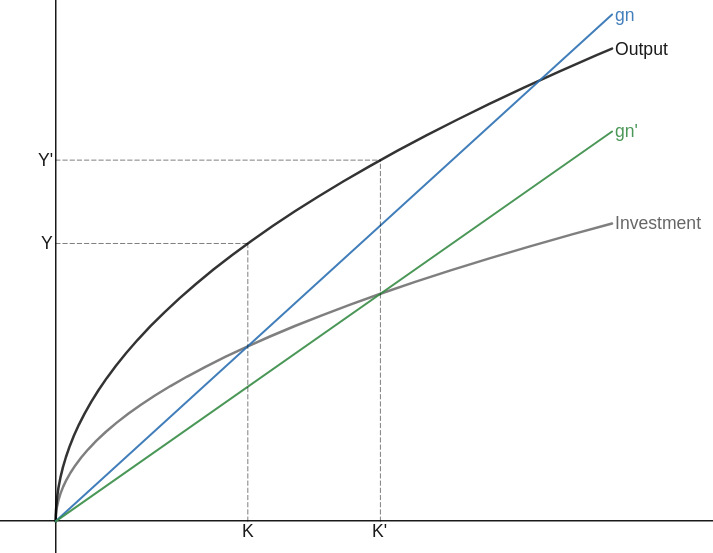
\includegraphics{/home/fontle/obsidian/Attachments/Pasted image 20230315151057.png}
\emph{(Beight-Welland, 2023)}

To conclude, we can see that a permanent decrease in population growth
would result in a increase in output per effective worker, and thus
overall GDP per capita. Furthermore, capital per worker increases since
if capital is accumulated at the same rate after the permanent
population decrease, more capital is available between fewer workers.

\hypertarget{bibliography-1}{%
\subsubsection{Bibliography}\label{bibliography-1}}

\begin{enumerate}
\tightlist
\item
  CFI. 2022, December 11, \emph{Technological Progress - Definition,
  Phases, How To Measure.} Corporatefinanceinstitute. {[}online{]}
  Available at:
  \url{https://corporatefinanceinstitute.com/resources/economics/technological-progress/}
  {[}Accessed 15 March. 2023{]}.
\item
  Blanchard, O \& Amighini, A \& Giavazzi, F. 2013,
  \emph{Macroeconomics: A European Perspective, Pearson Education UK,
  Harlow}. Available from: ProQuest Ebook Central. {[}15 March 2023{]}.
\item
  Beight-Welland, I. March 2023, \emph{Modelling Population Growth
  Change with the Solow Model}. Desmos. {[}online{]} Available at:
  \url{https://www.desmos.com/calculator/k48twmbzw2}
\end{enumerate}

\end{document}
